%%%%%%%%%%%%%%%%%%%%%%%%%%%%%%%%%%%%%%%%%
% HW Template
% LaTeX Template
% Version 1.0 (19/10/18)
% Modified by
% Erdem TUNA
% Halil TEMURTAŞ 
% Enes TAŞTAN 
%%%%%%%%%%%%%%%%%%%%%%%%%%%%%%%%%%%%%%%%%
%
%----------------------------------------------------------------------------------------
%	PACKAGES AND OTHER DOCUMENT CONFIGURATIONS
%----------------------------------------------------------------------------------------
\documentclass[a4paper,12pt]{article}
%-----packages------
\usepackage[a4paper, total={6.2in, 8.5in}]{geometry}
\usepackage[english]{babel}
\usepackage[utf8x]{inputenc}
\usepackage{amsmath}
\usepackage{graphicx}
\usepackage[colorinlistoftodos]{todonotes}
\usepackage{gensymb} % this could be problem
\usepackage{float}
\usepackage{fancyref}
\usepackage{subcaption}
\usepackage[toc,page]{appendix} %appendix package
\usepackage{xcolor}
\usepackage{listings}
\usepackage{xspace}
\usepackage{amssymb}
\usepackage{nicefrac}
\usepackage{gensymb}
\usepackage{fancyhdr}
\usepackage{blindtext}  % for dummy text, use \blindtext or \BlindText
\usepackage{lipsum}    % for dummy text, use \lipsum[3-56]
\usepackage[final]{pdfpages}  % pdf include
\usepackage{array} %allows more options in tables
\usepackage{pgfplots,pgf,tikz} %coding plots in latex
\usepackage{capt-of} % allows caption outside the figure environment
\usepackage[export]{adjustbox} %more options for adjusting the images
\usepackage{multicol,multirow,slashbox} % allows tables like table1
%\usepackage[hyperfootnotes=false]{hyperref} % clickable references
\usepackage{epstopdf} % useful when matlab is involved
%\usepackage{placeins} % prevents the text after figure to go above figure with \FloatBarrier 
%\usepackage{listingsutf8,mcode} %import .m or any other code file mcode is for matlab highlighting
\usepackage{steinmetz}

%-----end of packages

%-----specifications-----
\definecolor{mGreen}{rgb}{0,0.6,0} % for python
\definecolor{mGray}{rgb}{0.5,0.5,0.5}
\definecolor{mPurple}{rgb}{0.58,0,0.82}
\definecolor{mygreen}{RGB}{28,172,0} % color values Red, Green, Blue for matlab
\definecolor{mylilas}{RGB}{170,55,241}

\setcounter{secnumdepth}{5} % how many sectioning levels to assign numbers to
\setcounter{tocdepth}{5}    % how many sectioning levels to show in ToC

\lstdefinestyle{CStyle}{
	commentstyle=\color{mGreen},
	keywordstyle=\color{magenta},
	numberstyle=\tiny\color{mGray},
	stringstyle=\color{mPurple},
	basicstyle=\footnotesize,
	breakatwhitespace=false,         
	breaklines=true,
	frame=single,
	rulecolor=\color{black!40},                 
	captionpos=b,                    
	keepspaces=true,                 
	numbers=left,                    
	numbersep=5pt,                  
	showspaces=false,                
	showstringspaces=false,
	showtabs=false,                  
	tabsize=2,
	language=C
}

\lstset{language=Matlab,%
	%basicstyle=\color{red},
	breaklines=true,%
	frame=single,
	rulecolor=\color{black!40},
	morekeywords={matlab2tikz},
	keywordstyle=\color{blue},%
	morekeywords=[2]{1}, keywordstyle=[2]{\color{black}},
	identifierstyle=\color{black},%
	stringstyle=\color{mylilas},
	commentstyle=\color{mygreen},%
	showstringspaces=false,%without this there will be a symbol in the places where there is a space
	numbers=left,%
	numberstyle={\tiny \color{black}},% size of the numbers
	numbersep=9pt, % this defines how far the numbers are from the text
	emph=[1]{for,end,break},emphstyle=[1]\color{red}, %some words to emphasise
	%emph=[2]{word1,word2}, emphstyle=[2]{style},    
}


\tikzset{
	desicion/.style={
		diamond,
		draw,
		text width=4em,
		text badly centered,
		inner sep=0pt
	},
	block/.style={
		rectangle,
		draw,
		text width=10em,
		text centered,
		rounded corners
	},
	cloud/.style={
		draw,
		ellipse,
		minimum height=2em
	},
	descr/.style={
		fill=white,
		inner sep=2.5pt
	},
	connector/.style={
		-latex,
		font=\scriptsize
	},
	rectangle connector/.style={
		connector,
		to path={(\tikztostart) -- ++(#1,0pt) \tikztonodes |- (\tikztotarget) },
		pos=0.5
	},
	rectangle connector/.default=-2cm,
	straight connector/.style={
		connector,
		to path=--(\tikztotarget) \tikztonodes
	}
}

\tikzset{
	desicion/.style={
		diamond,
		draw,
		text width=4em,
		text badly centered,
		inner sep=0pt
	},
	block/.style={
		rectangle,
		draw,
		text width=10em,
		text centered,
		rounded corners
	},
	cloud/.style={
		draw,
		ellipse,
		minimum height=2em
	},
	descr/.style={
		fill=white,
		inner sep=2.5pt
	},
	connector/.style={
		-latex,
		font=\scriptsize
	},
	rectangle connector/.style={
		connector,
		to path={(\tikztostart) -- ++(#1,0pt) \tikztonodes |- (\tikztotarget) },
		pos=0.5
	},
	rectangle connector/.default=-2cm,
	straight connector/.style={
		connector,
		to path=--(\tikztotarget) \tikztonodes
	}
}
%-----end of specifications-----


%----commands----
\newcommand\nd{\textsuperscript{nd}\xspace}
\newcommand\rd{\textsuperscript{rd}\xspace}
\newcommand\nth{\textsuperscript{th}\xspace} %\th is taken already
\newcommand{\specialcell}[2][c]{ \begin{tabular}[#1]{@{}c@{}}#2\end{tabular}} % for too long table lines

\newcommand{\blankpage}{
	\- \\[9cm]	
	{ \centering \textit{This page intentionally left blank.} \par }
	\- \\[9cm]
}% For Blank Page

\makeatletter
\renewcommand\paragraph{\@startsection{paragraph}{4}{\z@}%
	{-2.5ex\@plus -1ex \@minus -.25ex}%
	{1.25ex \@plus .25ex}%
	{\normalfont\normalsize\bfseries}}
\makeatother
%-----end of commands-----


\pagestyle{fancy}
\fancyhead[LO,LE]{Halil TEMURTAŞ / 2094522 }
\fancyhead[RO,RE]{\today}
\fancyfoot[RO,RE]{
\includegraphics[width=2.7cm]{eelogo}}

\begin{document}
\begin{center}
	\textbf{\large EE430 Digital Signal Processing \\[0.2cm] HW 1} \\
\end{center}

\begin{enumerate}
	\item A DT $x[n]$ is obtained by sampling the $ x_c(t) = 4\sin(20000\pi 𝑡 + \frac{\pi}{13})$ at sampling rate  of $3~kHz$.
		
		\begin{enumerate}
			\item The same DT signal can be constructed by sampling the set of signals in a form
				$$ x_c(t) = 4\sin((20000+ 3000k)\pi 𝑡 + \frac{\pi}{13})~~,~~k=[-6,\infty)$$ 
			 or equivalently,
				$$  x_c(t) = 4\sin((2000+3000k)\pi 𝑡 + \frac{\pi}{13})~~,~~k=[0,\infty)$$
			\item Let $\Omega_0=2000$ for our signal, the sampled signal can be expressed as;
				$$	x[n]=4\sin(\Omega_0nT_s+\pi/3)	$$
			it should be equal to the signal sampled at $\widetilde{T_s} \triangleq T_s+\Delta T$ 
				$$	x[n]=4\sin(\Omega_0n\widetilde{T_s}+\pi/3)=4\sin(\Omega_0n(T_s+\Delta T)+\pi/3)	$$
			To satisfy the equation $\Omega_0n\Delta T$ should be equal to $k2\pi$ and knowing that 
				$$	\Omega_0=2\pi f_0	$$
				$$	\Delta t=\frac{k}{f_0} = kT_0	$$
				$$ \widetilde{T_s}=T_s+\Delta T $$
			using the equations above, the new set sampling frequencies that give the same $x[n]$ can be found as follows;
				$$	\boxed{ f_s'=\frac{f_s f_0}{f_0+kf_s} }~~,~~k=0,1,2...	$$
			for our case $f_0=1000$ and $f_s=3000$, from there other sampling frequencies that yield $x[n]$ from $x_c(t)$ can be calculated.
			
			 
		\end{enumerate}

		
	
	\item For any DT sinusoidal $cos(w_0n+\phi)$ or complex exponential $e^{w_0n+\phi}$ to be periodic with $N$, it has to satisfy the following,
		$$	w_0n=k2\pi	$$
		or equivalently,
		$$\boxed{N=\frac{2\pi}{w_0}k} ~~,~~ k,N \in \mathcal{Z} 	$$
		
		For the given functions,
		\begin{itemize}
			\item $\sin(1.74\pi n+3.1)$, periodic with $N_1=\cfrac{2\pi}{1.74\pi}k=100$ with $k=87$
			\item $\sin(1.74\pi n+31\pi)$, periodic with $N_2=\cfrac{2\pi}{1.74\pi}k=100$ with $k=87$
			\item $\cos(15.74\pi n+\cfrac{3\pi}{8})$, periodic with $N_3=\cfrac{2\pi}{15.74\pi}k=100$ with $k=787$
			\item $\cos(\sqrt{\pi} n)$, not periodic since there is no integer $k$ that makes $N_4=\cfrac{2\pi}{\sqrt{\pi}} k$ an integer
			\item $\cos(\pi \sqrt{\pi} n)$, not periodic since there is no integer $k$ that makes $N_5=\cfrac{2\pi}{\pi \sqrt{\pi}}k$ an integer
			\item $\cos(\pi \sqrt{2} n)$, not periodic since there is no integer $k$ that makes $N_6=\cfrac{2\pi}{\pi \sqrt{2} }k$ an integer
			
		\end{itemize}
		
	 
	
	\item For any linear system, the output can be calculated as,
		$$	y[n]=x[n]*h[n]\triangleq\sum_{k=-\infty}^{\infty} x[k]h[n-k]	$$		
		Response to a shifted response, can be calculated as follows,
		$$	h_k[n]=(u-k)u[n-k]=\delta[n-k]*h[n]	$$
		$$	\delta[n-k]*h[n]\triangleq\sum_{a=-\infty}^{\infty} \delta [a-k]h[n-a]=h[n-a] 	$$
		$$ h[n-a]|_{a=k} \equiv h[n-k]=h_k[n]=(n-k)u[n-k] $$
		From there, the impulse response $h[n]$ can be found as,
		$$ h[n]=nu[n] $$
		Thus, $y[n]$ for any input can be found as follows,
		$$	y[n]=x[n]*h[n]\triangleq\sum_{k=-\infty}^{\infty} x[k](n-k)u[n-k]$$
		$$	\boxed{	y[n]=\sum_{k=-\infty}^{n} x[k](n-k)	} $$
		To check time-invariance, let us find $y[n-m$ and the output $y_1[n]$ for an input $x_1[n]\triangleq x[n-m]$
		$$	y[n-m]=	\sum_{k=-\infty}^{\infty} x[k]h[n-m-k] $$
		$$ y_1[n]= x[n-m]*h[n] \triangleq \sum_{k=-\infty}^{\infty} x[k-m] h[n-k] $$		
		Letting $ \widetilde{k} \triangleq k-m $, $k=m+\widetilde{k}$
		$$ y_1[n] = \sum_{\widetilde{k}=-\infty}^{\infty} x[\widetilde{k}]h[n-m-\widetilde{k}]		$$
		It can be easily seen that $y[n-m]=y_1[n]$. Thus, the system is \textbf{Time-Invariant}.
	
	\item The system basically up-samples the system, by adding the average of two consecutive samples between these samples. An example Input/Output pair for the system can be seen at \textit{Figure~\ref{fig:ioq4}}.
	
		\begin{figure}[H]
			\centering
			\setlength{\unitlength}{\textwidth} 
			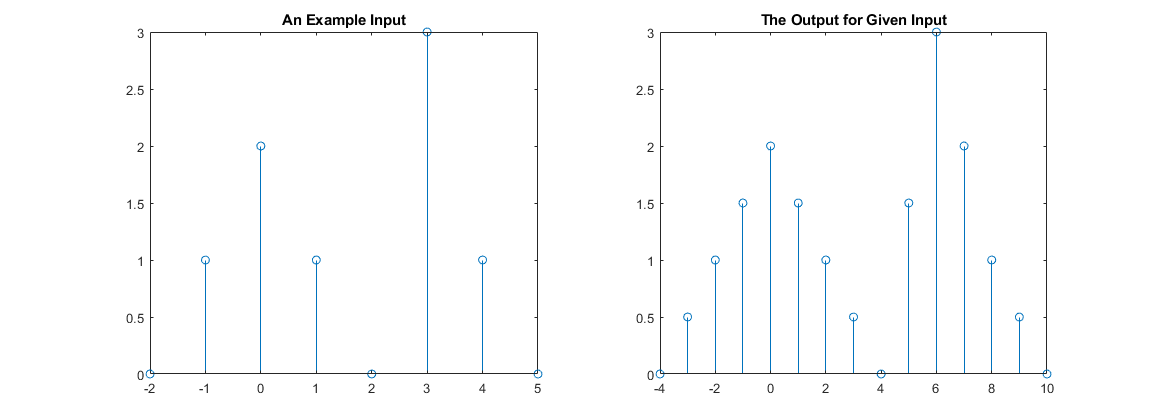
\includegraphics[width=1.0\unitlength]{q4}
			\caption{\label{fig:ioq4}An Example Input/Output Pair }
		\end{figure}
		
		\begin{itemize}
			\item For linearity, let us check the output $y[n]$ for the input $x[n]=ax_1[n]+bx_2[n]$
				$$  y[n] = 
     		\begin{cases}
     			\cfrac{x[n]}{2} ~~ if ~~ n~~is~~even \\
     			\cfrac{x[\cfrac{n-1}{2}]+x[\cfrac{n+1}{2}]}{2} ~~ if ~~ n~~is~~odd\\
     		\end{cases}	$$
     		
     		$$  y[n] = 
     		\begin{cases}
     			a\cfrac{x_1[n]}{2}+b\cfrac{x_2[n]}{2} ~~ n~~is~~even \\
     			
     			a\cfrac{x_1[\cfrac{n-1}{2}]+x_1[\cfrac{n+1}{2}]}{2}+b\cfrac{x_2[\cfrac{n-1}{2}]+x_2[\cfrac{n+1}{2}]}{2} ~~ if ~~ n~~is~~odd\\
     		\end{cases}	$$

		Let us also find $y_1[n]$ and $y_2[n]$ for $x_1[n]$ and $x_2[n]$ respectively,
		
			$$  y_1[n] = 
     		\begin{cases}
     			\cfrac{x_1[n]}{2} ~~ n~~is~~even \\
     			
     			\cfrac{x_1[\cfrac{n-1}{2}]+x_1[\cfrac{n+1}{2}]}{2}~~ if ~~ n~~is~~odd\\
     		\end{cases}	$$
     		$$  y_2[n] = 
     		\begin{cases}
     			\cfrac{x_2[n]}{2} ~~ n~~is~~even \\
     			
     			\cfrac{x_2[\cfrac{n-1}{2}]+x_2[\cfrac{n+1}{2}]}{2} ~~ if ~~ n~~is~~odd\\
     		\end{cases}	$$

		It can be clearly seen that $y[n]=ay_1[n]+y_2[n]$ for $x[n]=ax_1[n]+bx_2[n]$. Thus, the system is \textbf{Linear}.
		
			\item For time invariance, let us check $y[n-m]$ and $y_1[n]$ for the $x_1[n]=x[n-m]$
				$$  y[n-m] = 
     		\begin{cases}
     			\cfrac{x[n-m]}{2} ~~ if ~~ (n-m)~~is~~even \\
     			\cfrac{x[\cfrac{n-m-1}{2}]+x[\cfrac{n-m+1}{2}]}{2} ~~ if ~~ (n-m)~~is~~odd\\
     		\end{cases}	$$
     		$$  y_1[n] = 
     		\begin{cases}
     			\cfrac{x_1[n]}{2} ~~ if ~~ n~~is~~even \\
     			\cfrac{x_1[\cfrac{n-1}{2}]+x_1[\cfrac{n+1}{2}]}{2} ~~ if ~~ n~~is~~odd\\
     		\end{cases}	$$
     		$$  y_1[n] = 
     		\begin{cases}
     			\cfrac{x[n-m]}{2} ~~ if ~~ n~~is~~even \\
     			\cfrac{x[\cfrac{n-m-1}{2}]+x[\cfrac{n-m+1}{2}]}{2} ~~ if ~~ n~~is~~odd\\
     		\end{cases}	$$
     		
     		Due to condition difference $y[n-m] \neq y_[n]$. For different $m$, the result changes. Thus, the system is \textbf{not Time-Invariant}.
				  
		\end{itemize}
		
	
	\item Let us check stability and causality for the following systems;
		\begin{itemize}
			\item 
			$$ y[n]=2^{\delta [n+1]}+x[n-3]$$ 
			The system is \textbf{not casual} since the impulse response $h[n] \neq 0$ as $n<0$;
			$$ h[n]=2^{\delta [n+1]}+\delta [n-3] $$
			For BIBO stability, let us assume $|x[n]|<\beta_x<\infty $ and check $|y[n]|$;
			$$	|y[n]|=|2^{\delta [n+1]}+x[n-3]|=|c+x[n]|=\beta_y<\infty	$$
			where $c$ and $\beta_y$ are finite constants, thus, the system is \textbf{Stable}. 
			 
			
			\item $$	y[n] = 
     		\begin{cases}
     			y[-\delta [n-1]]+x[n-3] ~~ if ~~ n>0 \\
     			2^n x[n-3] ~~ if ~~ n\leq 0\\
     		\end{cases}	$$
     		The system is \textbf{Casual} since the impulse response $h[n]=0$ as $n<0$;     		
     		$$	h[n] = 
     		\begin{cases}
     			h[-\delta [n-1]]+\delta [n-3] ~~ if ~~ n>0 \\
     			2^n \delta[n-3] ~~ if ~~ n\leq 0\\
     		\end{cases}		$$
     		For BIBO stability, let us assume $|x[n]|<\beta_x<\infty $ and check $|y[n]|$;
     		$$	|y[n]| = 
     		\begin{cases}
     			|y[-\delta [n-1]]+x[n-3]| ~~ if ~~ n>0 \\
     			|2^n x[n-3]| ~~ if ~~ n\leq 0\\
     		\end{cases}	$$
     		Let us assume $|y[n]|<\beta_z<\infty$. Checking the two conditions, the assumption holds, thus, it can be seen that the system is \textbf{Stable}. 
		\end{itemize}
	
	\item 
		$$	y[n]=x[n]*x[n]=\sum_{k=-\infty}^{\infty} x[k]x[n-k]	$$
		If the first non-zero element of $x[n]$ is $x[-6]=-3$ and the last non-zero element of $x[n]$ is equal to $x[24]=-4$, the first and last non-zero elements of $y[n]$ will be $y[-12]$ from $(-6=6+n)$ and $y[48]$ from $(24=-24+n)$. These values can be calculated from the formula above as,
			$$ \boxed{y[-12]=x[-6]x[-6]=9} $$ 
			$$ \boxed{y[48]=x[24]x[24]=16} $$ 
			
		
		
	
	\item Let us calculate $y[n]$ as $n \to \infty$, given that $x[n]=u[n]$ and $h[n]=3{(\frac{1}{2})}^nu[n]+2{(\frac{1}{3})}^{n-1}u[n] $
		$$	y[n]=x[n]*h[n]=\sum_{k=-\infty}^{\infty} x[k]h[n-k]	$$
		$$	y[n]=\sum_{k=-\infty}^{\infty} u[k](3{(\frac{1}{2})}^{(n-k)}u[n-k]+2{(\frac{1}{3})}^{n-k-1}u[n-k])	$$
		$$	y[n]=\sum_{k=0}^{n} 3{(\frac{1}{2})}^{(n-k)}+6{(\frac{1}{3})}^{(n-k)}	$$
		with simple change of variables, let $m\triangleq n-k$
		$$	=\sum_{m=n}^{0} 3{(\frac{1}{2})}^m +6{(\frac{1}{3})}^m	$$
		or as $n \to \inf$
		$$ y[n]= \sum_{m=0}^{\infty} 3{(\frac{1}{2})}^m +6{(\frac{1}{3})}^m $$
		$$	\boxed{\lim_{n \to \infty} y[n]=3\cfrac{1}{1-1/2}-6\cfrac{1}{1-1/3}=-3}	$$
	\item Let us analyse the system $y[n]-\frac{1}{2}y[n-1]=x[n]-x[n-1]+x[n-2]$
	Assume homogeneous system $y[n]-\frac{1}{2}y[n-1]=0$ and solve it for finding homogeneous solution $y_h[n]$.
	
	$$	y[n]-\frac{1}{2}y[n-1]=0 ~~~,~~~with~~~y_h[n]=Ar^n	$$
	$$	Ar^n-\frac{A}{2}r^{n-1}=0	$$	
	$$ 	Ar^{n-1}(r-\frac{1}{2})=0	$$
	$$	\boxed {r=1/2} $$
	Thus, the homogeneous solution will be in the form of $A{(\frac{1}{2})}^{n}$,
	Let us now find the impulse response of the system $y_1[n]-\frac{1}{2}y_1[n-1]=x[n]$, the homogeneous solution will also satisfy this system and the impulse response will be also in form of  $y_h[n]$
	$$	h_1[n]-\frac{1}{2}h_1[n-1]=\delta [n] $$
	We also know that $h_1[n]$ will be in the for $Ar^nu[n]$ since the system is casual. To find $A$, let us calculate $h_1[n]$ at $n=0$.
	$$  h_1[0]=\frac{1}{2}h[-1]+\delta [0]=1=A{(\frac{1}{2})}^0=A $$
	Thus, we have found the impulse response of the system $y_1[n]-\frac{1}{2}y_1[n-1]=x[n]$ as
	$$ \boxed {h_1[n] = {( \frac{1}{2})}^nu[n]} $$
		\begin{enumerate}
			\item Due to lineartity of the system, the impulse response of the system \\ $y[n]-\frac{1}{2}y[n-1]=x[n]-x[n-1]+x[n-2]$ will be superposition of the impulse response $h_1[n]$;
			$$ h[n]=h_1[n]-h_1[n-1]+h_1[n-2] $$
			$$ h[n]={\frac{1}{2}}^nu[n]-{\frac{1}{2}}^{n-1}u[n-1]+{\frac{1}{2}}^{n-2}u[n-2] $$
			$$ 	h[n]={\frac{1}{2}}^n(u[n]-2u[n-1]+4u[n-2])	$$
			$$ \boxed{	h[n]={\frac{1}{2}}(\delta [n]-\delta [n-1] +3u[n-2]) }$$
			\item Frequency response $H(e^{jw})$ can be found as;
				$$	H(e^{jw})=\sum_{n=\infty}^{\infty}h[n]e^{-jwn}	$$
				$$	H(e^{jw})=\sum_{n=\infty}^{\infty}{(\frac{1}{2})}^ne^{-jwn}\delta [n]-\sum_{n=\infty}^{\infty} {(\frac{1}{2})}^ne^{-jwn}\delta [n-1] +3\sum_{n=\infty}^{\infty}{(\frac{1}{2})}^ne^{-jwn}u[n-2] $$
				$$	H(e^{jw})= 1-\frac{1}{2}e^{jw}+3\sum_{n=2}^{\infty}{(\frac{e^{-jw}}{2})}^n$$				
				$$	H(e^{jw})=-2-2e^{-jw}+\frac{6}{2-e^{-jw}} \-~~if~~~|\frac{e^{-jw}}{2}|<1$$
				$$	\boxed {H(e^{jw})=-2-2e^{-jw}+\frac{6}{2-e^{-jw}} ~~if~~~\-\pi<w<\pi}	$$
			\item 	To use freqz command, we have to compete the Z-transform of the system,
			$$	Y(z)-\frac{1}{2}Y(z)z^{-1}=X(z)-X(z)z^{-1}+X(z)z^{-2} $$
			$$	\boxed {H(z) \triangleq \cfrac{Y(z)}{X(z)} = \cfrac{1-z^{-1}+z^{-2}}{1-\frac{1}{2}z^{-1}} } $$
			The result can be seen at \textit{Figure~\ref{fig:8c}}.
				\begin{figure}[H]
					\centering
					\setlength{\unitlength}{\textwidth} 
					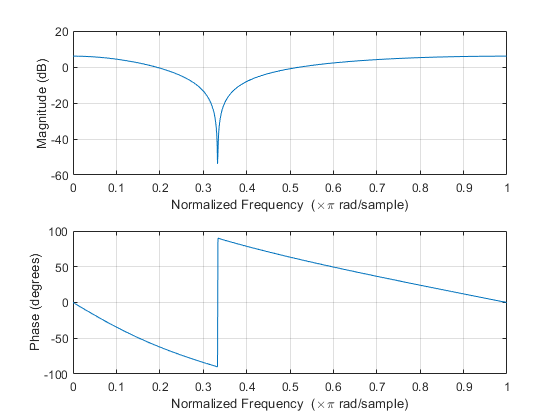
\includegraphics[width=1.0\unitlength]{8c}
					\caption{\label{fig:8c}Magnitude and Phase of Frequency Response }
				\end{figure}
				\lstinputlisting[language=Matlab]{q8.m}
			\item 	Since we have $H(e^{jw})$, we can find $y[n]$ from
				$$	Y(e^{jw})=X(e^{jw})H(e^{jw})	$$
				instead of convolution, for that we need to find $X(e^{jw})$ first. Given that $x[n]=\cos(\frac{\pi}{3}n)+\sin(\frac{\pi}{2}n+\frac{\pi}{4})$
				$$ x[n]=\cos(\frac{\pi}{3}n)+\sin(\frac{\pi}{2}n)\cos(\frac{\pi}{4})+\cos(\frac{\pi}{2}n)\sin(\frac{\pi}{4})) $$
				$$ x[n]=\cos(\frac{\pi}{3}n)+\sin(\frac{\pi}{2}n)\frac{1}{\sqrt{2}}+\cos(\frac{\pi}{2}n)\frac{1}{\sqrt{2}}) $$				
				\-\\[1cm]
				$$ X(e^{jw})=\pi\left[\delta [w-\frac{\pi}{3}]+\delta [w+\frac{\pi}{3}]\right]-\frac{j\pi}{\sqrt{2}}\left[\delta [w-\frac{\pi}{2}]-\delta [w+\frac{\pi}{2}]\right] $$ $$ +\frac{\pi}{\sqrt{2}}\left[\delta [w-\frac{\pi}{2}]+\delta [w+\frac{\pi}{2}]\right] $$

				$$ X(e^{jw})=\pi\left[\delta [w-\frac{\pi}{3}]+\delta [w+\frac{\pi}{3}]\right]+\frac{\pi}{\sqrt{2}}(1-j)\left[\delta [w-\frac{\pi}{2}]\right] $$ $$ +\frac{\pi}{\sqrt{2}}(1+j)\left[\delta [w+\frac{\pi}{2}]\right] $$
				
				$$ 	Y(e^{jw})=X(e^{jw})H(e^{jw})	$$

				$$	Y(e^{jw})=\pi\left[-2-2e^{-j\pi/3}+\frac{6}{2-e^{-j\pi/3}}\right]\delta [w-\frac{\pi}{3}]	$$	
				$$	+\pi\left[-2-2e^{-j\pi/3}+\frac{6}{2-e^{-j\pi/3}}\right]\delta [w+\frac{\pi}{3}]  $$
				$$ +\frac{\pi}{\sqrt{2}}(1-j)\left[-2-2e^{-j\pi/2}+\frac{6}{2-e^{-j\pi/2}}\right]\delta [w-\frac{\pi}{2}] $$ 
				$$+\frac{\pi}{\sqrt{2}}(1+j)\left[-2-2e^{j\pi/2}+\frac{6}{2-e^{j\pi/2}}\right]\delta [w+\frac{\pi}{2}]$$

				by some computation, the term above becomes
				$$	\boxed {Y(e^{jw})=\frac{\pi}{\sqrt{2}}\left[\frac{6}{5}+j\frac{2}{5}\right]\delta [w-\frac{\pi}{2}] + \frac{\pi}{\sqrt{2}}\left[\frac{6}{5}-j\frac{2}{5}\right]\delta [w+\frac{\pi}{2}]} $$
				the $y[n]$ can be found to be as
				$$	y[n]=\frac{\pi}{\sqrt{2}}\left[\frac{6}{5}+j\frac{2}{5}\right]\frac{1}{2\pi}e^{j\frac{\pi}{2}n} + \frac{\pi}{\sqrt{2}}\left[\frac{6}{5}-j\frac{2}{5}\right]\frac{1}{2\pi}e^{-j\frac{\pi}{2}n}	$$
				by also some computation, the term above becomes
				$$\boxed{	y[n]=	\frac{1}{\sqrt{2}}\left[\frac{3}{5}+j\frac{1}{5}\right]e^{j\frac{\pi}{2}n} + \frac{1}{\sqrt{2}}\left[\frac{3}{5}-j\frac{1}{5}\right]e^{-j\frac{\pi}{2}n} }$$		
			\item 	Let us analyse $H(e^{jw})$ found,		
			$$ H(e^{jw})=-2-2e^{-jw}+\frac{6}{2-e^{-jw}} $$	
			$$ H^*(e^{j(2\pi-w)})={\left(-2-2e^{-j(2\pi-w)}+\frac{6}{2-e^{-j(2\pi-w)}}\right)}^* $$
			$$ H^*(e^{j(2\pi-w)})={\left(-2-2e^{-j2\pi}e^{jw)}+\frac{6}{2-e^{-j2\pi}e^{jw)}}\right)}^* $$	
			$$ H^*(e^{j(2\pi-w)})={\left(-2-2e^{jw)}+\frac{6}{2-2e^{jw)}}\right)}^* $$	
			$$\boxed { H^*(e^{j(2\pi-w)})=-2-2e^{-jw)}+\frac{6}{2-2e^{-jw)}}} $$	
			which obliviously equal to the $H(e^{jw})$ as asked in the question.
			
		\end{enumerate}
	
	\item 
		
		\begin{enumerate}
			\item Since $x[n]$ is a real sequence, magnitude of its frequency response must be even symmetric and phase plot of its frequency response must be odd symmetric. 
			\item With given $x[n]$, $x_c[n]$ and $x_s[n]$, the DTFTs can be found by convolution in the frequency domain,
				$$	x_c[n]=\cos(\frac{\pi}{5}n) x[n]$$
				$$	X_c(e^{jw})=X(e^{jw})*\mathcal{F}\{\cos(\frac{\pi}{5}n)\} $$
				$$ \mathcal{F}\{\cos(\frac{\pi}{5}n)\}=\pi\left[\delta [w-\frac{\pi}{5}]+\delta [w+\frac{\pi}{5}]\right] $$
				$$\boxed{	X_c(e^{jw})= \pi\left[X(e^{j(w+\pi/5)})+X(e^{j(w-\pi/5)})\right] }$$
				$$	x_s[n]=\sin(\frac{\pi}{5}n) x[n]$$
				$$	X_s(e^{jw})=X(e^{jw})*\mathcal{F}\{\sin(\frac{\pi}{5}n)\} $$
				$$ \mathcal{F}\{\sin(\frac{\pi}{5}n)\}=-j\pi\left[\delta [w-\frac{\pi}{5}]-\delta [w+\frac{\pi}{5}]\right] $$
				$$\boxed{	X_s(e^{jw})= -j\pi\left[X(e^{j(w+\pi/5)})-X(e^{j(w-\pi/5)})\right] }$$
			\item
		\end{enumerate}
	
	\item It is known that, the DTFT of $x[n]$ can be calculated as follows;
		$$	X(e^{jw})=\sum_{-\infty}^{\infty}x[n]e^{-jwn}	$$
		\begin{enumerate}
			\item 
				$$\boxed{	X(e^{jw})|_{w=0}=\sum_{-\infty}^{\infty}x[n]=6	}$$
			\item
				$$	X(e^{jw})|_{w=\pi}=\sum_{-\infty}^{\infty}x[n]e^{-j\pi n}$$
				$$\boxed{	X(e^{jw})|_{w=\pi}=\sum_{-\infty}^{\infty}x[n]{(-1)}^{ n}=2	}$$
			\item Since x[n] is symmetric about n=2, the signal has linear phase
			$$	X(e^{jw})=A(w)e^{-j2w}	$$
			$A(w)$ is a zero phase(real) function of w. Thus,
			$$	\phase{X(e^{jw})}=-2w~~,~~-\pi \leq w\leq \pi	$$
			\item Knowing that $	\int_{\infty}^{\infty}X(e^{jw}e^{-jwn})dw=2\pi x[n]	$, for $n=0$, equations becomes what we desired
			$$\boxed{	\int_{\infty}^{\infty}X(e^{jw})dw= 2\pi x[0]=4}$$
			\item Assume $x_1[n]$ whose DTFT is $X(e^{-jw})$.
			$$ X(e^{jw})=\sum_{-\infty}^{\infty} x[n]e^{jwn}=\sum_{-\infty}^{\infty} x[-n]e^{-jwn}=\sum_{-\infty}^{\infty} x_1[n]e^{-jwn} $$
			Thus, it can be seen that,	
			$$\boxed{	x_1[n]=x[-n]	}$$
			$x[-n]$ can be seen from \textit{Figure~\ref{fig:q10a}}.
				\begin{figure}[H]
					\centering
					\setlength{\unitlength}{\textwidth} 
					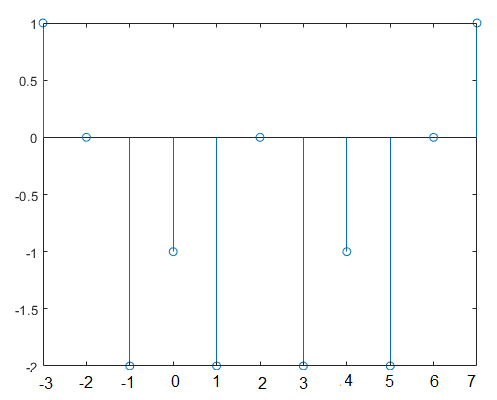
\includegraphics[width=0.6\unitlength]{q10a}
					\caption{\label{fig:q10a} $x[-n]$  }
				\end{figure}
			\item Remembering $ X(e^{jw})=A(w)e^{-j2w}	$, real part of $X(e^{jw})$ can be written as
			$$	X_R(e^{jw})=A(w)\cos(2w) $$
			$$	X_R(e^{jw})=\frac{1}{2}A(w)\left( e^{j2w}+e^{-j2w} \right)	$$
			$$	x_R[n]=\mathcal{F}^{-1}\{X_R(e^{jw}) \}	$$
			$$	x_R[n]=\frac{1}{2}a[n+2]+\frac{1}{2}a[n-2]	$$
			$$\boxed{	x_R[n]=\frac{1}{2}x[n+4]+\frac{1}{2}x[n]	}$$
			$x_R[n]$ can be seen from \textit{Figure~\ref{fig:q10b}}.
				\begin{figure}[H]
					\centering
					\setlength{\unitlength}{\textwidth} 
					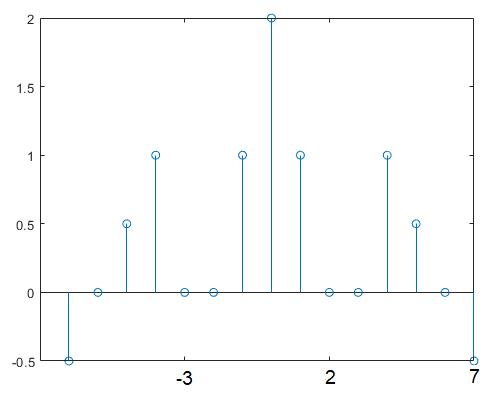
\includegraphics[width=0.6\unitlength]{q10b}
					\caption{\label{fig:q10b} $x_R[n]$  }
				\end{figure}
		\end{enumerate}
	\item 		
		\begin{enumerate}
			\item From the given informations
		\begin{itemize}
			\item $h[n]=0$ for $n<0$, causality,
			\item $h[n]$ is real, FT is conjugate symmetric,
			\item $h[n+1$ is even, real FT	
		\end{itemize}
		From above, , it can be understood that, $h[n]$ is 3-length long, thus, it is finite-duration.
			\item Notice that, $h[n]$ has three elements and symmetric, so, let us assume $h[0]=h[2]=a$ and $h[1]=b$.
			
			From extra informations
				\begin{itemize}
					\item  $2a^2+b^2=2$, Parseval's Theorem
					\item  $2a-b=0 $
				\end{itemize}
				Solving the equations found above, \boxed{a=\frac{\pm 1}{\sqrt{3}}} and \boxed{b=\frac{\pm 2}{\sqrt{3}}}. 
		\end{enumerate}
		$$\boxed{	h[0]=h[2]=\frac{\pm 1}{\sqrt{3}}~~,~~h[1]=\frac{\pm 2}{\sqrt{3}}	}$$
	
	\item It can be observed from the question that $X(e^{jw})$ is real and
	$$ Y(e^{jw})= \begin{cases}
     			-jX(e^{jw}) ~~,~~ 0<w<\pi \\
     			+jX(e^{jw}) ~~,~~ -\pi<w<0\\
     		\end{cases} $$
     		It is also given that $w[n]=x[n]+jy[n]$, thus,
     		$$ W(e^{jw})=+jY(e^{jw})$$ 
			$$\boxed{ W(e^{jw})= \begin{cases}
     			2X(e^{jw})~~, ~~ 0<w<\pi \\
     			0 ~~,~~ -\pi<w<0\\
     		\end{cases} }$$
     		$W(e^{jw})$ can be seen from \textit{Figure~\ref{fig:q10a}}.
     		\begin{figure}[H]
					\centering
					\setlength{\unitlength}{\textwidth} 
					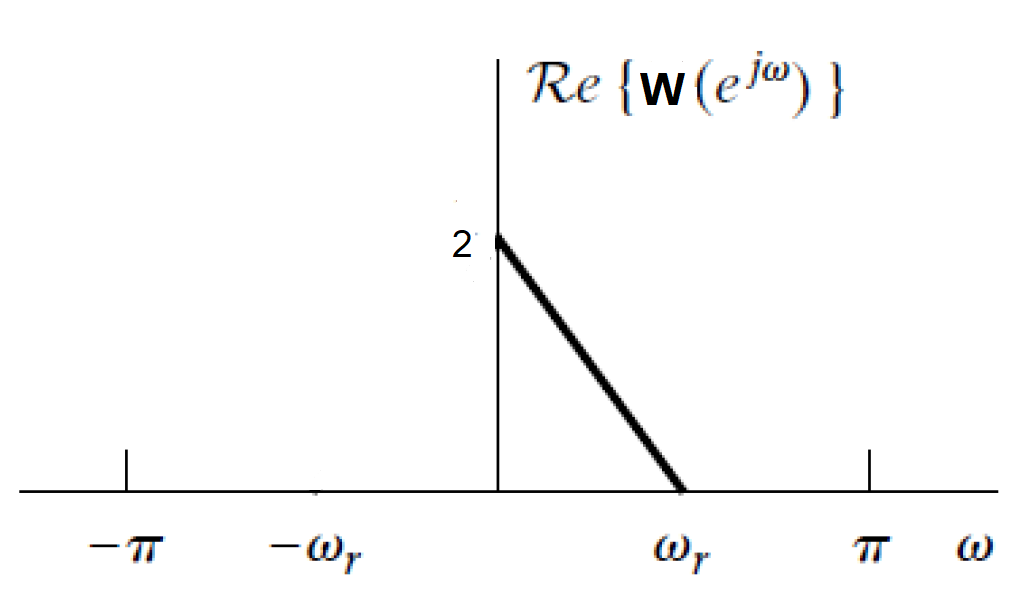
\includegraphics[width=0.6\unitlength]{q11a}
					\caption{\label{fig:q11a} $W(e^{jw})$  }
				\end{figure}
	\-\\[2cm]
	\item {[MATLAB]} 
		
		\begin{enumerate}
			\item \lstinputlisting[language=Matlab,firstline=1, lastline=19]{q13.m}
			\item  The result of 'conv' function can be seen at \textit{Figure~\ref{fig:q13b2}}.
				\begin{figure}[H]
					\centering
					\setlength{\unitlength}{\textwidth} 
					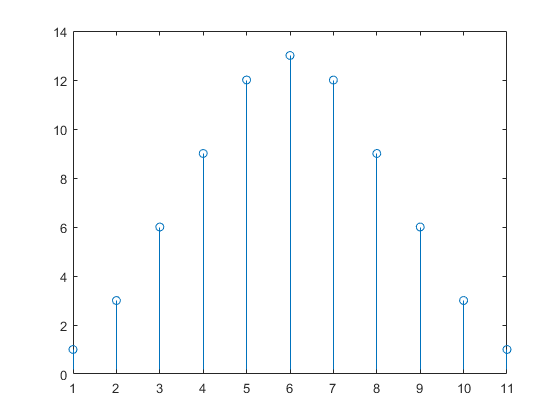
\includegraphics[width=0.6\unitlength]{q13b2}
					\caption{\label{fig:q13b2} The result of 'conv' function  }
				\end{figure}  \-\\
				\lstinputlisting[language=Matlab,firstline=23, lastline=30]{q13.m}
			\item Magnitude and phase response of the filter $h[n]$ can be seen at \textit{Figure~\ref{fig:q13c}}.
				\begin{figure}[H]
					\centering
					\setlength{\unitlength}{\textwidth} 
					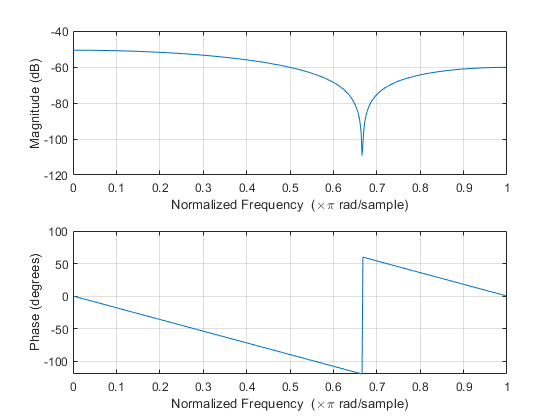
\includegraphics[width=0.9\unitlength]{q13c}
					\caption{\label{fig:q13c} Magnitude and phase response of the filter $h[n]$ }
				\end{figure} 
				\lstinputlisting[language=Matlab,firstline=33, lastline=34]{q13.m} \-\\[1cm]
			\item The result for the $h_2[n]*x[n]$  can be seen at \textit{Figure~\ref{fig:q13d1}}.
				\begin{figure}[H]
					\centering
					\setlength{\unitlength}{\textwidth} 
					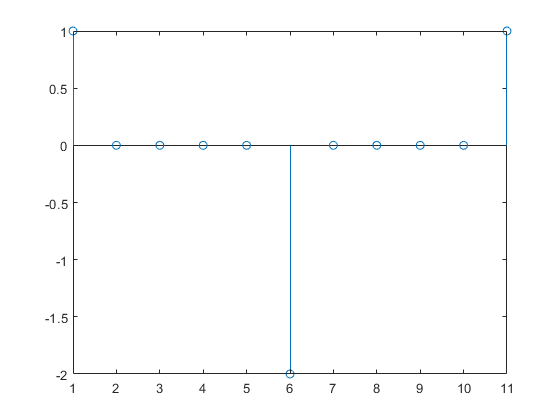
\includegraphics[width=0.6\unitlength]{q13d1}
					\caption{\label{fig:q13d1} $h_2[n]*x[n]$  }
				\end{figure}
				\lstinputlisting[language=Matlab,firstline=37, lastline=41]{q13.m} \-\\[8cm]
			\item Magnitude and phase response of the filter $h_2[n]$  can be seen at \textit{Figure~\ref{fig:q13e}}.
				\begin{figure}[H]
					\centering
					\setlength{\unitlength}{\textwidth} 
					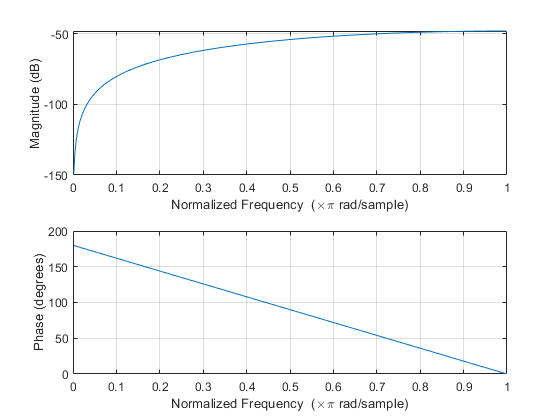
\includegraphics[width=0.9\unitlength]{q13e}
					\caption{\label{fig:q13e} Magnitude and phase response of the filter $h_2[n]$  }
				\end{figure}
				\lstinputlisting[language=Matlab,firstline=44, lastline=45]{q13.m} \-\\[6cm]
			\item Magnitude and phase response of $z[n]$ can be seen at \textit{Figure~\ref{fig:q13f}}.
				\begin{figure}[H]
					\centering
					\setlength{\unitlength}{\textwidth} 
					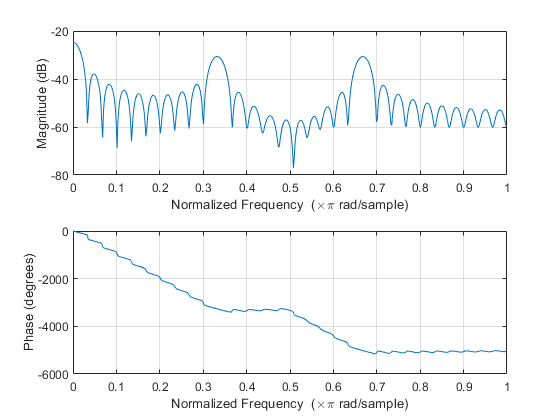
\includegraphics[width=0.9\unitlength]{q13f}
					\caption{\label{fig:q13f} Magnitude and phase response of the  $z[n]$  }
				\end{figure}
				\lstinputlisting[language=Matlab,firstline=47, lastline=59]{q13.m} \-\\[1cm]
			\item Magnitude and phase response of $y[n]=z[n]*h[n]$ can be seen at \textit{Figure~\ref{fig:q13f}}.
				\begin{figure}[H]
					\centering
					\setlength{\unitlength}{\textwidth} 
					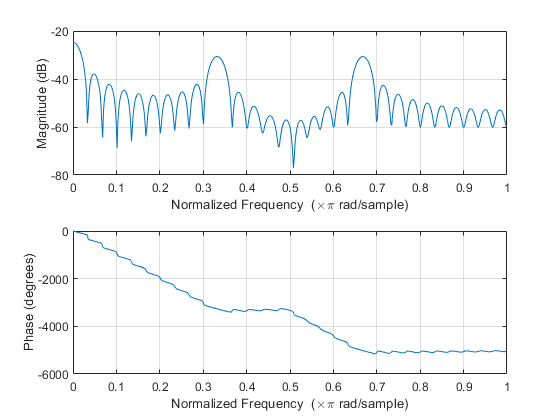
\includegraphics[width=0.9\unitlength]{q13f}
					\caption{\label{fig:q13f} Magnitude and phase response of the  $y[n]$  }
				\end{figure}
				\lstinputlisting[language=Matlab,firstline=62, lastline=65]{q13.m}
			
		\end{enumerate}
		
	\end{enumerate}
	
%\begin{appendices}
%		\lstinputlisting[language=Matlab,firstline=23, lastline=59]{q13.m}
%\end{appendices}

\end{document}

%----samples------
%\begin{itemize}
%\item Item
%\item Item
%\end{itemize}

%\begin{figure}[H]
%\center
%\setlength{\unitlength}{\textwidth} 
%\includegraphics[width=0.7\unitlength]{images/logo1}
%\caption{\label{fig:logo}Logo }
%\end{figure}

%\begin{figure}[H]
%	\setlength{\unitlength}{\textwidth} 
%	\centering
%	\begin{subfigure}{.5\textwidth}
%  		\centering
%  		\includegraphics[width=0.48\unitlength]{images/logo1}
%  		\caption{\label{fig:logo1}Logo1 }
%	\end{subfigure}%
%	\begin{subfigure}{.5\textwidth}
%  		\centering
%		\includegraphics[width=0.48\unitlength]{images/logo2}
%  		\caption{\label{fig:logo2}Logo2}
%	\end{subfigure}
%\caption{\label{fig:calisandegree} Small Logos   }
%\end{figure}
	
%\begin{table}[H]
%  \centering
% 
%    \begin{tabular}{c|c|c}
%       $$A$$ & $$B$$ & $$C$$ \\ \hline
%       1 & 2 & 3  \\ \hline
%       2 & 3 & 4  \\ \hline
%       3 & 4 & 5  \\ \hline
%       4 & 5 & 6  
%      
%  \end{tabular}
%  \caption{table}
%  \label{tab:table}
%\end{table}
	
%\begin{table}[H]
%  \centering
% 
%    \begin{tabular}{c|c|c}
%       \backslashbox{$A$}{$a$} & $$\specialcell{ Average deviation \\ after subtracting out the  \\ frequency error }$$ & $$C$$ \\ \hline
%       \multirow{2}{*}{1} & 2 & 3  \\ \cline{2-3}
%        & 3 & 4  \\ \hline
%       3 & \multicolumn{2}{c}{4}  \\ \hline
%       4 & 5 & 6  
%      
%  \end{tabular}
%  \caption{table}
%  \label{tab:table}
%\end{table}
%-----end of samples-----